\documentclass{jss}
\usepackage[T1]{fontenc}

\usepackage[bold]{otf}

\usepackage{amsmath,amssymb}
\newcommand{\Rset}{\mathbf R}
\usepackage{amsthm}
\newtheorem*{cooperativepatrollingproblem}{協力警邏問題}
\usepackage[dvipdfmx]{graphicx}
\newcommand{\figdir}{../figures}

%%%%%%%%%%%%%%%%%%%%%%%%%%%%%%%%%%%%%%%%%%%%%
% タイトル
%%%%%%%%%%%%%%%%%%%%%%%%%%%%%%%%%%%%%%%%%%%%%
\title{%
  {\bfseries\LARGE 複数の巡査の協力による指定地点の警邏について}\\
  % 
  {\bfseries\Large Multi-agent Cooperative Patrolling of Designated Points on Graphs}
}

%%%%%%%%%%%%%%%%%%%%%%%%%%%%%%%%%%%%%%%%%%%%%
% 著者・所属(共著の場合.発表者に○印)
%%%%%%%%%%%%%%%%%%%%%%%%%%%%%%%%%%%%%%%%%%%%%
\author{%
  \presenter % 発表者の○印
  河村 彰星\\
  九州大学
  \\[6pt]
  Akitoshi Kawamura\\
  Kyushu University\\
%  kawamura@inf.kyushu-u.ac.jp\\
  \and
  能城 秀彬\\
  東京大学
  \\[6pt]
  Hideaki Noshiro\\
  University of Tokyo\\
}

%%%%%%%%%%%%%%%%%%%%%%%%%%%%%%%%%%%%%%%%%%%%%
% 著者・所属(単著の場合)
%%%%%%%%%%%%%%%%%%%%%%%%%%%%%%%%%%%%%%%%%%%%%
%\author{%
%スケジューリング 太郎\\
%△△大学
%\\[5mm]
%Taro Scheduling\\
%Anonymous University\\
%taro@anonymous-u.ac.jp\\
%}

%%%%%%%%%%%%%%%%%%%%%%%%%%%%%%%%%%%%%%%%%%%%%
% 英文概要
%%%%%%%%%%%%%%%%%%%%%%%%%%%%%%%%%%%%%%%%%%%%%
\abstract{%
We are given an undirected graph with edge lengths, and want to patrol it using several mobile agents, each of which can move along the edges with maximum speed $1$.  Each vertex~$v$ has an \emph{idle time} $q _v$ and a \emph{profit} $p _v$, and we want to maximize the sum of $p _v$ for vertices~$v$ that are visited at least once in every time period of length~$q _v$.  This problem has been studied by Coene et al., but they assumed that each vertex should be visited often enough by a single agent.  We remove this assumption, and show that for some simple graphs, the problem is efficiently solvable if the idle time $q _v$ are equal.  We also analyze the setting where instead of the idle times $q _v$, we specify the exact times at which to visit each $v$ periodically. 
}

\begin{document}
\maketitle

%%%%%%%%%%%%%%%%%%%%%%%%%%%%%%%%%%%%%%%%%%%%%
% ここから本文
%%%%%%%%%%%%%%%%%%%%%%%%%%%%%%%%%%%%%%%%%%%%%

\section{問題}

所与の領域を1人または複数の巡査が動き回り,
その領域内の指定された場所を十分な頻度で訪れることを
警邏(patrolling)という\cite{coene2011charlemagne, czyzowicz2011boundary}.


本稿では,与えられた距離空間$U$内を速さ$1$以下の巡査$m$人が動きまわることにより,
集合$V \subseteq U$に属する多くの点に十分な頻度で訪れるという目標を考える.
すなわち次の問題である.

巡査$i \in \{1, \ldots, m\}$の$U$上の運行$a _i \colon \Rset \to U$とは,
各時刻$t \in \Rset$における位置$a _i (t) \in U$を定めており,
任意の時刻$s$,$t \in \Rset$に対し$a _i (s)$と$a _i (t)$の距離が$\lvert s - t \rvert$を超えないものをいう.
巡査$m$人による$U$上の運行とは,
全巡査の運行を定めた組
$A = (a _1, \dots, a _m)$をいう.
運行$A$%
% $A = (a _i) _{i \in \{1, \ldots, m\}}$
が点$v \in U$を間隔$q \geq 0$で警備するとは,
長さ$q$のどの時間区間にも
いずれかの巡査が$v$を少くとも一度は訪れる
(任意の時刻$t \in \Rset$に対して
巡査$i$と時刻$\tau \in [t, t + q)$が存在し
$a _i (\tau) = v$)ことをいう.

$U$の有限な部分集合$V$があり,$V$の各点には利得および許容訪問間隔と呼ばれる非負整数が定まっている.
運行$A$が点集合$W \subseteq V$を警邏するとは,各点$v \in W$に対し,
$A$が$v$をその許容訪問間隔で警備することをいう.

\begin{cooperativepatrollingproblem}
    巡査の人数$m$と距離空間$U$内の点集合$V$および
    $V$の各点の利得と許容訪問間隔が
    与えられたとき,
    警邏可能な頂点集合のうち利得の和が最大となるものを求めよ.
\end{cooperativepatrollingproblem}

距離空間$U$といっても,$V$の点どうしの測地距離のみが重要である.
そこでこの問題の入力は,
$V$を頂点集合とし辺に非負整数の長さがついた無向グラフと考えることにする.

\section{背景}

この問題は,巡査が一人かつ
全頂点の利得と許容訪問間隔が等しい場合でも,
ハミルトン路問題からの帰着により
NP困難である\cite[Theorem~8]{coene2011charlemagne}.
そこでグラフの形状を限ったときを調べる.

一つの頂点が複数の巡査の訪問により警備され得ることに注意されたい(図\ref{figure: cooperative}左).
\begin{figure}
  \begin{center}
    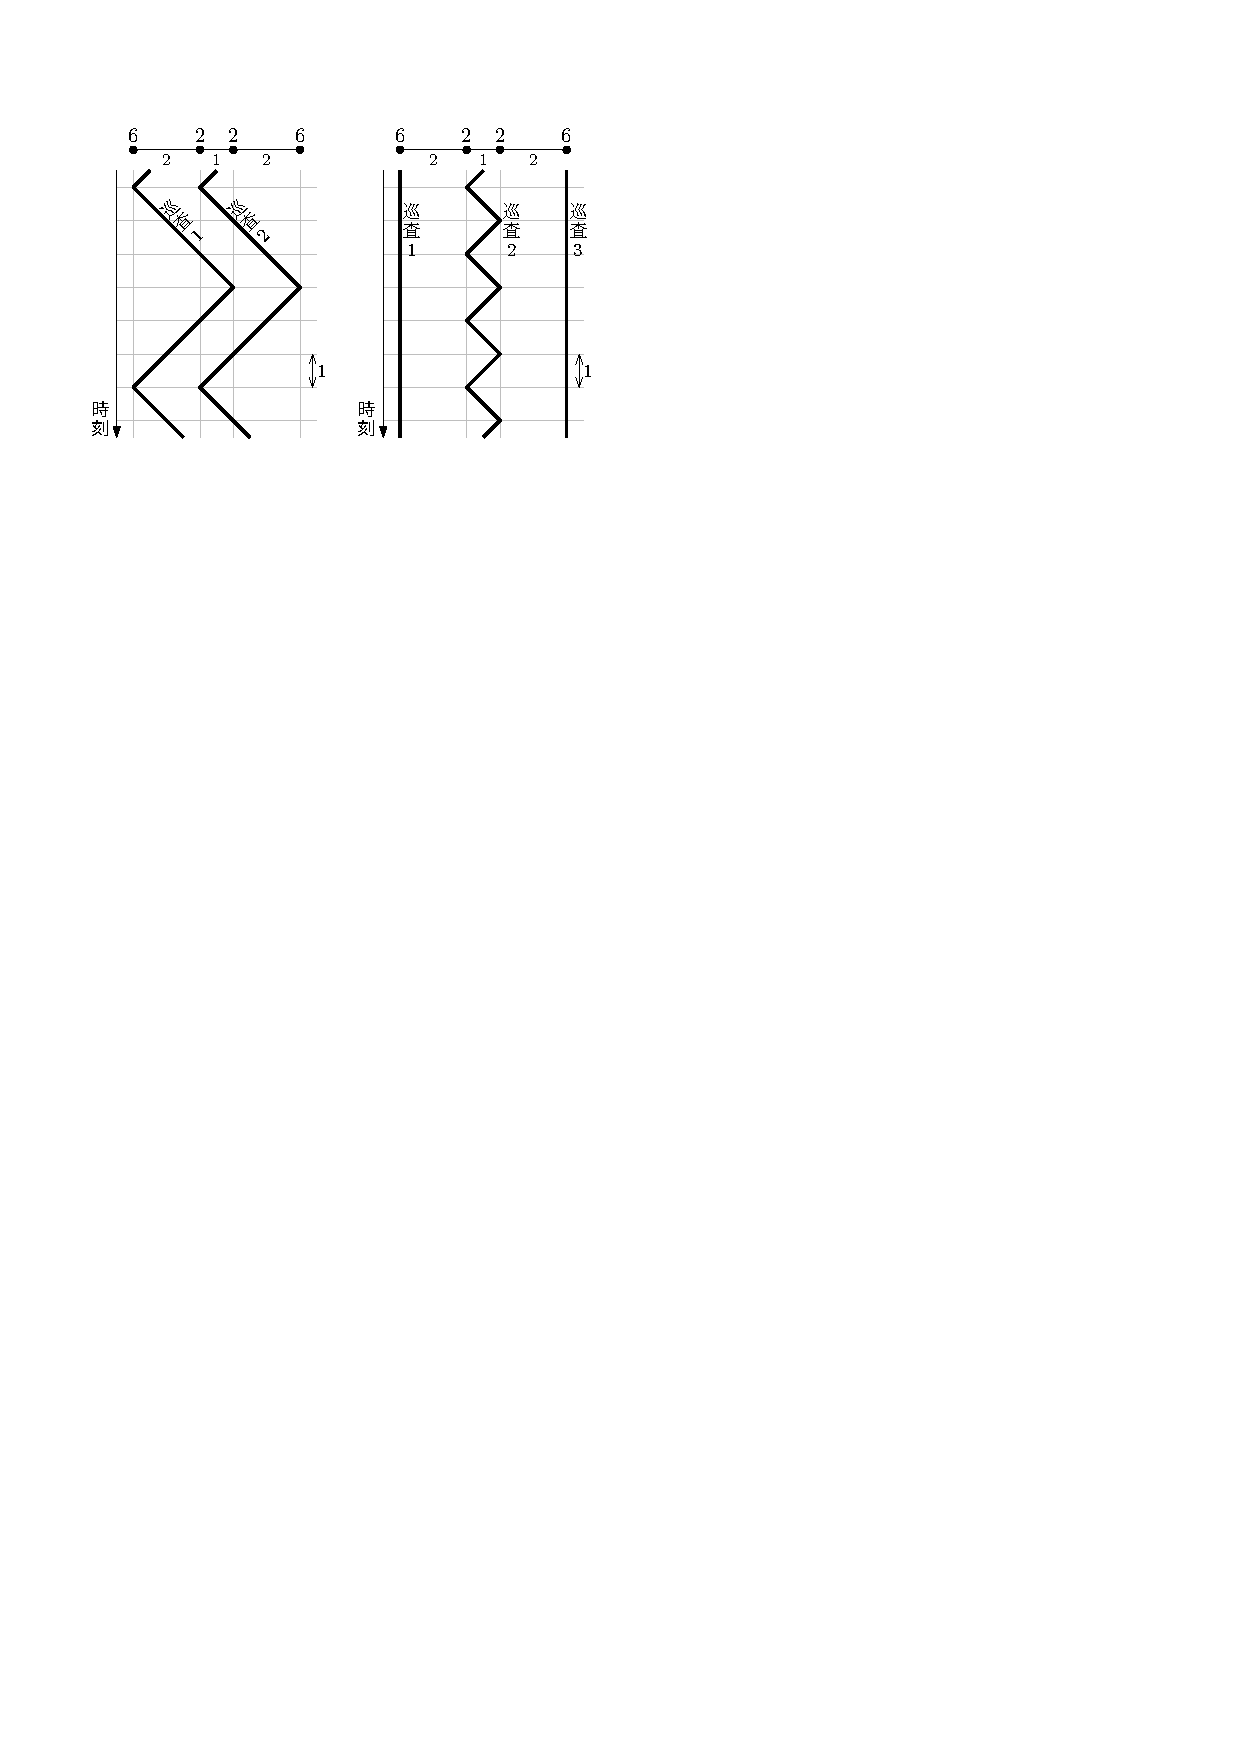
\includegraphics[scale=0.9]{\figdir/cooperative.pdf}
    \caption{図の上部に描かれている四点からなるグラフの全頂点を警邏する二つの運行.
      頂点と辺に書かれた数は,それぞれ許容訪問間隔と距離である.
      左図の運行では二人の巡査が協力して中央の二点を間隔$2$で警備している.
      これを禁じ,各点がいずれかの巡査により単独警備されることを求める場合は,
      右図のように三人の巡査を要する.}
    \label{figure: cooperative}
  \end{center}
\end{figure}
Coeneら\cite{coene2011charlemagne}は似た問題を扱っているが,
このような協力を許さず,
図\ref{figure: cooperative}右のように
各頂点を専ら一人の巡査が「担当」することを要求している.
つまり,各頂点$v \in W$が単独警備される(すなわち
或る一人の巡査がおり,
その巡査のみの運行が$\{v\}$を警邏する)ことを要求しているのである.
対比のため本稿ではこの問題を非協力警備問題と呼ぶことにする
(\cite{coene2011charlemagne}ではMPLPPと称している).
Coeneら\cite{coene2011charlemagne}の諸結果においては,
この非協力という限定が,
多項式時間算法の設計にも困難性の証明にも重要な役割を果している.
本研究ではこの限定を外した場合を調べた.

本稿ではグラフ$G$の形状として
線分,星と,枝の長さがすべて等しい完全グラフの3種類を扱うこととし
(図\ref{figure: graph_classes}),
以降はそれぞれを Line, Star, Unitと呼ぶ.
\begin{figure}
  \begin{center}
    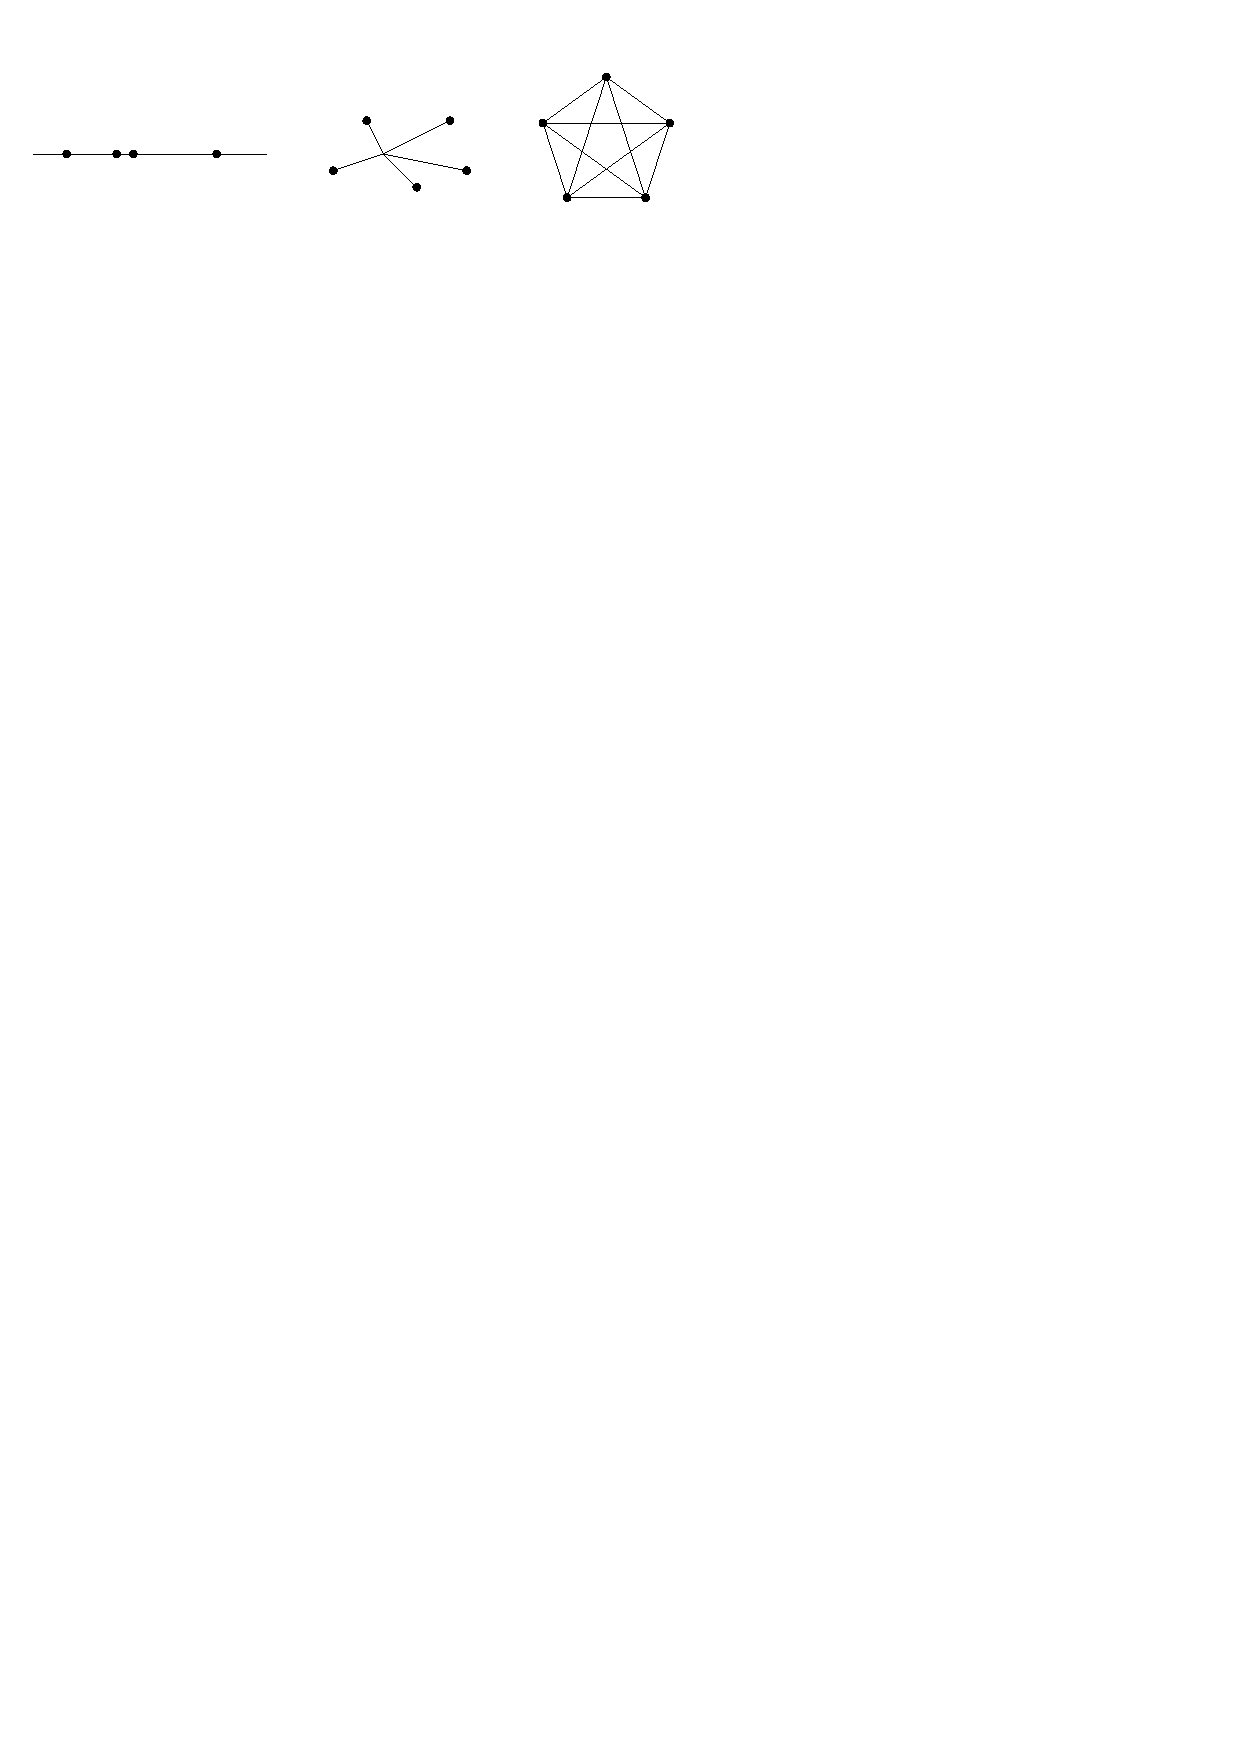
\includegraphics[scale=0.8]{\figdir/graph_classes.pdf}
    \caption{本研究ではLine(左),Star(中),Unit(右,但し各辺の長さが等しい)を扱う.Starは葉のみを警備の対象とする(中央の点は移動の途中で使うのみであり,訪問間隔は定められていない).}
    \label{figure: graph_classes}
  \end{center}
\end{figure}
Starでは葉のみに許容訪問間隔が定められている(中心は警備の対象としない).
Unitは,その各辺の長さを$d$とすると,
同じ頂点数で辺の長さがすべて$d/2$というStarの特別な場合と考えることができる.

\section{結果}

協力警邏問題について,以下の結果を得た.
\begin{itemize}
\item 
Lineでは,
非協力警邏問題は
動的計画法により多項式時間で解けることが
示されていた\cite[Theorem~11]{coene2011charlemagne}が,
その正しさは非協力という設定に強く依存している.
本研究では協力警邏問題について,
全頂点の許容訪問間隔が等しい場合には多項式時間で解けることを示す.
\item
Starでは,
全頂点の利得と許容訪問間隔がすべて等しい場合に限っても,
非協力警邏問題はNP困難であることが示されていた\cite[Theorem~10]{coene2011charlemagne}.
本研究では,この場合の協力警邏問題は多項式時間で解けるという興味深い結果を得た.
なお利得または許容訪問間隔を一般にすると,
巡査が一人であっても(したがって協力・非協力に関わらず)
NP困難であることがわかっている\cite[Theorems 5 and 6]{coene2011charlemagne}.
\item 
Unitでは,
全頂点の許容訪問間隔が等しい場合は
協力警邏問題が多項式時間で解けることがわかった.
Starでは全頂点の許容訪問間隔が等しくても利得が一般だとNP困難になるので,
これによりUnitはStarよりも簡単に解ける場合となっていることがわかる.
\end{itemize}

LineとUnitについては
許容訪問間隔が一般の場合については
多項式時間アルゴリズムやNP困難性を示すのが難しかったため,
許容訪問間隔の代わりに「厳密訪問間隔」というものを考え,
最初の訪問時刻から厳密訪問間隔ごとの時刻ちょうどに訪問し続けること
を警備の条件とする問題も考えた.
これは\cite{kawamura2015simple}に関係の深い設定であり,
類似の手法により,
Unitにおいて巡査が一人の場合でも警邏問題がNP困難であるなどの結果を得た.

本稿に挙げた結果の一部はコンピュテーション研究会で
発表した\cite{kenkyukai}.
残りの証明を含めた完全な論文は近日中に発表予定である.
本研究は旭硝子財団および科研費17K19960の助成を受けた.

\begin{thebibliography}{1}

  \small

\bibitem{kenkyukai}
河村,能城.\textgt{複数の巡査による指定地点の警邏について}.
電子情報通信学会コンピュテーション研究会.徳島県徳島市,平成28年9月.

\bibitem{coene2011charlemagne}
S.~Coene, F.\,C.\,R.~Spieksma, and G.\,J. Woeginger.
\newblock Charlemagne's challenge: the periodic latency problem.
\newblock {\em Operations research}, 59(3), pp.~674--683, 2011.


\bibitem{czyzowicz2011boundary}
J.~Czyzowicz, L.~G{\k{a}}sieniec, A.~Kosowski, and E.~Kranakis.
\newblock Boundary patrolling by mobile agents with distinct maximal speeds.
\newblock In {\it Proc.\ 19th Annual European Symposium on Algorithms} (ESA), LNCS~6942, pp.~701--712, 2011. 

\bibitem{kawamura2015simple}
A.~Kawamura and M.~Soejima.
\newblock Simple strategies versus optimal schedules in multi-agent patrolling.
\newblock In \emph{Proc.\ Ninth International Conference on Algorithms and Complexity} (CIAC), LNCS~9079, pp.~261--273, 2015.

\end{thebibliography}


\end{document}
